\documentclass{article}\usepackage[]{graphicx}\usepackage[]{color}
% maxwidth is the original width if it is less than linewidth
% otherwise use linewidth (to make sure the graphics do not exceed the margin)
\makeatletter
\def\maxwidth{ %
  \ifdim\Gin@nat@width>\linewidth
    \linewidth
  \else
    \Gin@nat@width
  \fi
}
\makeatother

\definecolor{fgcolor}{rgb}{0.345, 0.345, 0.345}
\newcommand{\hlnum}[1]{\textcolor[rgb]{0.686,0.059,0.569}{#1}}%
\newcommand{\hlstr}[1]{\textcolor[rgb]{0.192,0.494,0.8}{#1}}%
\newcommand{\hlcom}[1]{\textcolor[rgb]{0.678,0.584,0.686}{\textit{#1}}}%
\newcommand{\hlopt}[1]{\textcolor[rgb]{0,0,0}{#1}}%
\newcommand{\hlstd}[1]{\textcolor[rgb]{0.345,0.345,0.345}{#1}}%
\newcommand{\hlkwa}[1]{\textcolor[rgb]{0.161,0.373,0.58}{\textbf{#1}}}%
\newcommand{\hlkwb}[1]{\textcolor[rgb]{0.69,0.353,0.396}{#1}}%
\newcommand{\hlkwc}[1]{\textcolor[rgb]{0.333,0.667,0.333}{#1}}%
\newcommand{\hlkwd}[1]{\textcolor[rgb]{0.737,0.353,0.396}{\textbf{#1}}}%
\let\hlipl\hlkwb

\usepackage{framed}
\makeatletter
\newenvironment{kframe}{%
 \def\at@end@of@kframe{}%
 \ifinner\ifhmode%
  \def\at@end@of@kframe{\end{minipage}}%
  \begin{minipage}{\columnwidth}%
 \fi\fi%
 \def\FrameCommand##1{\hskip\@totalleftmargin \hskip-\fboxsep
 \colorbox{shadecolor}{##1}\hskip-\fboxsep
     % There is no \\@totalrightmargin, so:
     \hskip-\linewidth \hskip-\@totalleftmargin \hskip\columnwidth}%
 \MakeFramed {\advance\hsize-\width
   \@totalleftmargin\z@ \linewidth\hsize
   \@setminipage}}%
 {\par\unskip\endMakeFramed%
 \at@end@of@kframe}
\makeatother

\definecolor{shadecolor}{rgb}{.97, .97, .97}
\definecolor{messagecolor}{rgb}{0, 0, 0}
\definecolor{warningcolor}{rgb}{1, 0, 1}
\definecolor{errorcolor}{rgb}{1, 0, 0}
\newenvironment{knitrout}{}{} % an empty environment to be redefined in TeX

\usepackage{alltt}
%Required: You must have these
\usepackage{graphicx}
\usepackage{tabularx}
\usepackage{natbib}

\usepackage{array}
\usepackage{amsmath}
%\usepackage[backend=bibtex]{biblatex}
\setkeys{Gin}{width=0.8\textwidth}
%\setlength{\captionmargin}{30pt}
\setlength{\abovecaptionskip}{10pt}
\setlength{\belowcaptionskip}{10pt}
\topmargin -1.5cm 
\oddsidemargin -0.04cm 
\evensidemargin -0.04cm 
\textwidth 16.59cm
\textheight 23.94cm 
\parskip 7.2pt 
\renewcommand{\baselinestretch}{1.2} 	
\parindent 0pt


\bibliographystyle{..//refs/styles/besjournals.bst}
%\usepackage{xr-hyper}
\usepackage{hyperref}
\title{Ecological drivers of hysteranthous flowering vary across taxonomic scale in the North American cherries (\texit{Prunus spp.}) or
Aridity and pollinator attraction drive hysteranthous flowering in the North American cherries (\texit{Prunus spp.})}
\IfFileExists{upquote.sty}{\usepackage{upquote}}{}
\begin{document}
\maketitle


\section*{Introduction}
\noindent Woody perennials have the unique ability among plants to seasonally begin reproduction prior to vegetative growth \citep{}. This flowering-first phenological sequence known as hysteranthy, proteranthy or precocious flowering is particularly common in temperate forests around the globe \citep{}. A number of studies suggest that this flower-leaf sequences (FLSs) are under selection, and that flowering first has functional significance \citep{}.

\noindent The most common, and well-tested explanation for the evolution of hysteranthy is that it is adaptive for wind-pollination as leafless canopies increase wind speeds for pollen transport and reduce the likelihood of pollen interception on vegetation \citep{}. However, this hypothesis fails to address the prevalence of hysteranthous taxa that are biotically-pollinated. Approximately 30\% of species of Eastern temperate forests of North America flower before leafing out, and of those, approximately 20\% are biotically pollinated  \citep{}. Despite the pervasiveness of this phenological syndrome, direct tests of the function of hysteranthy in biotically pollinated taxa are exceedingly rare. \\

Yetm two major hypotheses regarding the functionality of hysteranthy pollinated taxa can be found in the literature, and each is associated with logical predictions about how hysteranthous flowering should other plant traits should co-vary. These hypotheses and their predictions can be used to guide further inquiry into the adaptive significance of hysteranthy.\\

The \textbf{water dynamics hypothesis} \citep{} suggests that hysteranthy is an adaptation to arid environments \citep{}, allowing for plant to partition the hydraulic demand of hydrated flowers and transpiring leaves across the growing season. If this is the case, this hypothesis predicts that hysteranthous species should be more commonly found in dry environments.  \\

The \textbf{pollinator visibility hypothesis} \citep{} suggests that hysteranthy is an adaptation to attract visually-foraging pollinators. If this is the case, this hypothesis predicts that hysteranthous species should invest less along other axes of pollinator attracting such as size of floral display or chemical attraction. \\

\noindent Others have suggested that hysteranthy is simply the by-product of selection for early flowering,and that variation in flower-leaf sequences among species is driven by developmental, physical or phylogenetic constraints than adaptive selection \citep{}. However, even this null hypothesis make testable predictions. If this is the case, hysteranthy should co-vary with other early-flowering associated traits like long fruit development periods or large fruit sizes \citep{} and the phylogenetic signal for hysteranthy should be strong.

\noindent However, there are two major methodological challenges to testing these predictions:\\

The first is that traits like aridity tolerance, pollinator attraction, and reproductive investment are the emergent product of a suite of biological traits \citep{}. Across the diversity of even just temperature woody plants, species may rely more or less heavily on any combination of these traits. For example, hysteranthy may contribute significantly to differences in aridity tolerance two species with similar root architecture, leaf characteristics and xylem anatomy, but matter much less when comparing deep rooted species to shallow rooted ones. Thus, in analyzing selective drivers of any trait at large taxonomic scales, unmeasured trait differences may obscure the estimated effects of the trait of interest.\\

This is a common problem in trait-based ecology, and one of the most promising solutions for understanding the functional significance of hysteranthy in woody plants is through character deconstruction \citep{}; comparing flower-leaf sequences variation for only a subset of taxa of shared phylogenetic and morphological character.   


The second challenge for robust testing of flower-first hypotheses is that most characterizations of flower-leaf phenological sequences are based on expert-opinion verbal descriptions(e.g. ``flowers before leaves" or ``flower before/with leaves"), which make comparisons across taxa, time and space difficult sensitive to observer bias (see, \citep{}). 

This problem can be overcome by adopting standardized quantitative measures of plant phenology for observational studies and applying them to historic data records. Herbarium records are an excellent source of data that can be leveraged for quantitative phenological measurements \citep{}, but have not be used widely to investigate variability of flower-leaf sequences variation among and within species.







there are several methodological challenges.


\begin{enumerate}
\item Unmeasured species difference compensate for measure traits
\item data quality based on expert opinion
\end{enumerate}






%<<>>=
%mich.data<-read.csv("..//..//sub_projs/MTSV_USFS/michdata_final.csv")
%table(mich.data$pro2,mich.data$Pollination)

%table(mich.data$pro)
%42/147
%table(mich.data$pro2)
%82/147

@



%Generally speaking, hysteranthy is unique and common in temperate forest. Seems functionial. The most common, and well tested, explaination is that is hysteranthy evolved for wind-pollination. However that doesn't explain its prevalence in biotically pollinated taxa. Quote some statistic based new phyt paper. Tests of the function on hysteranthy in biotically pollinated taxa are exceedingly rare in the literature,, but may be critial for predicting species responses to global change.

%While direct tests are limited, investegation of hysteranthy beneifit from a rich theoretical literature and several hypotheses have emerge.

%Review them briefly and make predictions
%\begin{enumerate}
%\item Drought adaptation: (could be plastic or selected) aridity in range
%\item insect visaibility: floral morphology
%\item Null functionality early flowering. Fruit size or phenology
%\item Phylogeny may also matter
%\end{enumerate}

%While each hypothesis generates testible predictions there are several methodological challenges.
%\begin{enumerate}
%\item Unmeasured species difference compensate for measure traits
%\item data quality based on expert opinion
%\end{enumerate}

%These issues could be over come with:
%\begin{enumerate}
%\item character deconstruction
%\item detailed quantitative measurements of flower leaf sequence phenology
%\end{enumerate}

%We do this:
%\begin{enumerate}
%\item Coarse analyses of the flower-leaf sequences of North American \textit{Prunus} species and their hypothesis relevant traits based on published data
%\item Higher resolution inquiry of the fLower-leaf sequences and associated character traits based on our own measurements from a century worth of herbaria samples on a section of the Prunus subgenus Prunocerasus the American plums
%\end{enumerate}

\section*{Methods}
\subsection{Descriptions of the genus, and section}
Say why they are ideal for this analyses
\subsection{Genus level analyses}
Data source\\
Methods for analysis\\

\subsection{Section level analyes}
Methods for herbaria measurements\\
Methods for analysis\\
\pagebreak

\section*{Results}

\section*{Discussion}
There will probably be things about taxonomic scale. Ie attraction showing up at the genus but not section level. Major discussion of why. \\
Pollinator attraction and drought tolerance are a suite of traits and we only measured one axis of them and even with character deconstruction this could matter\\
Mechanistic experiments would still be useful, ie does water limitation influence FLS plasticity
\newpage
\section*{Figures}
    \begin{figure}[h!]
    \centering
 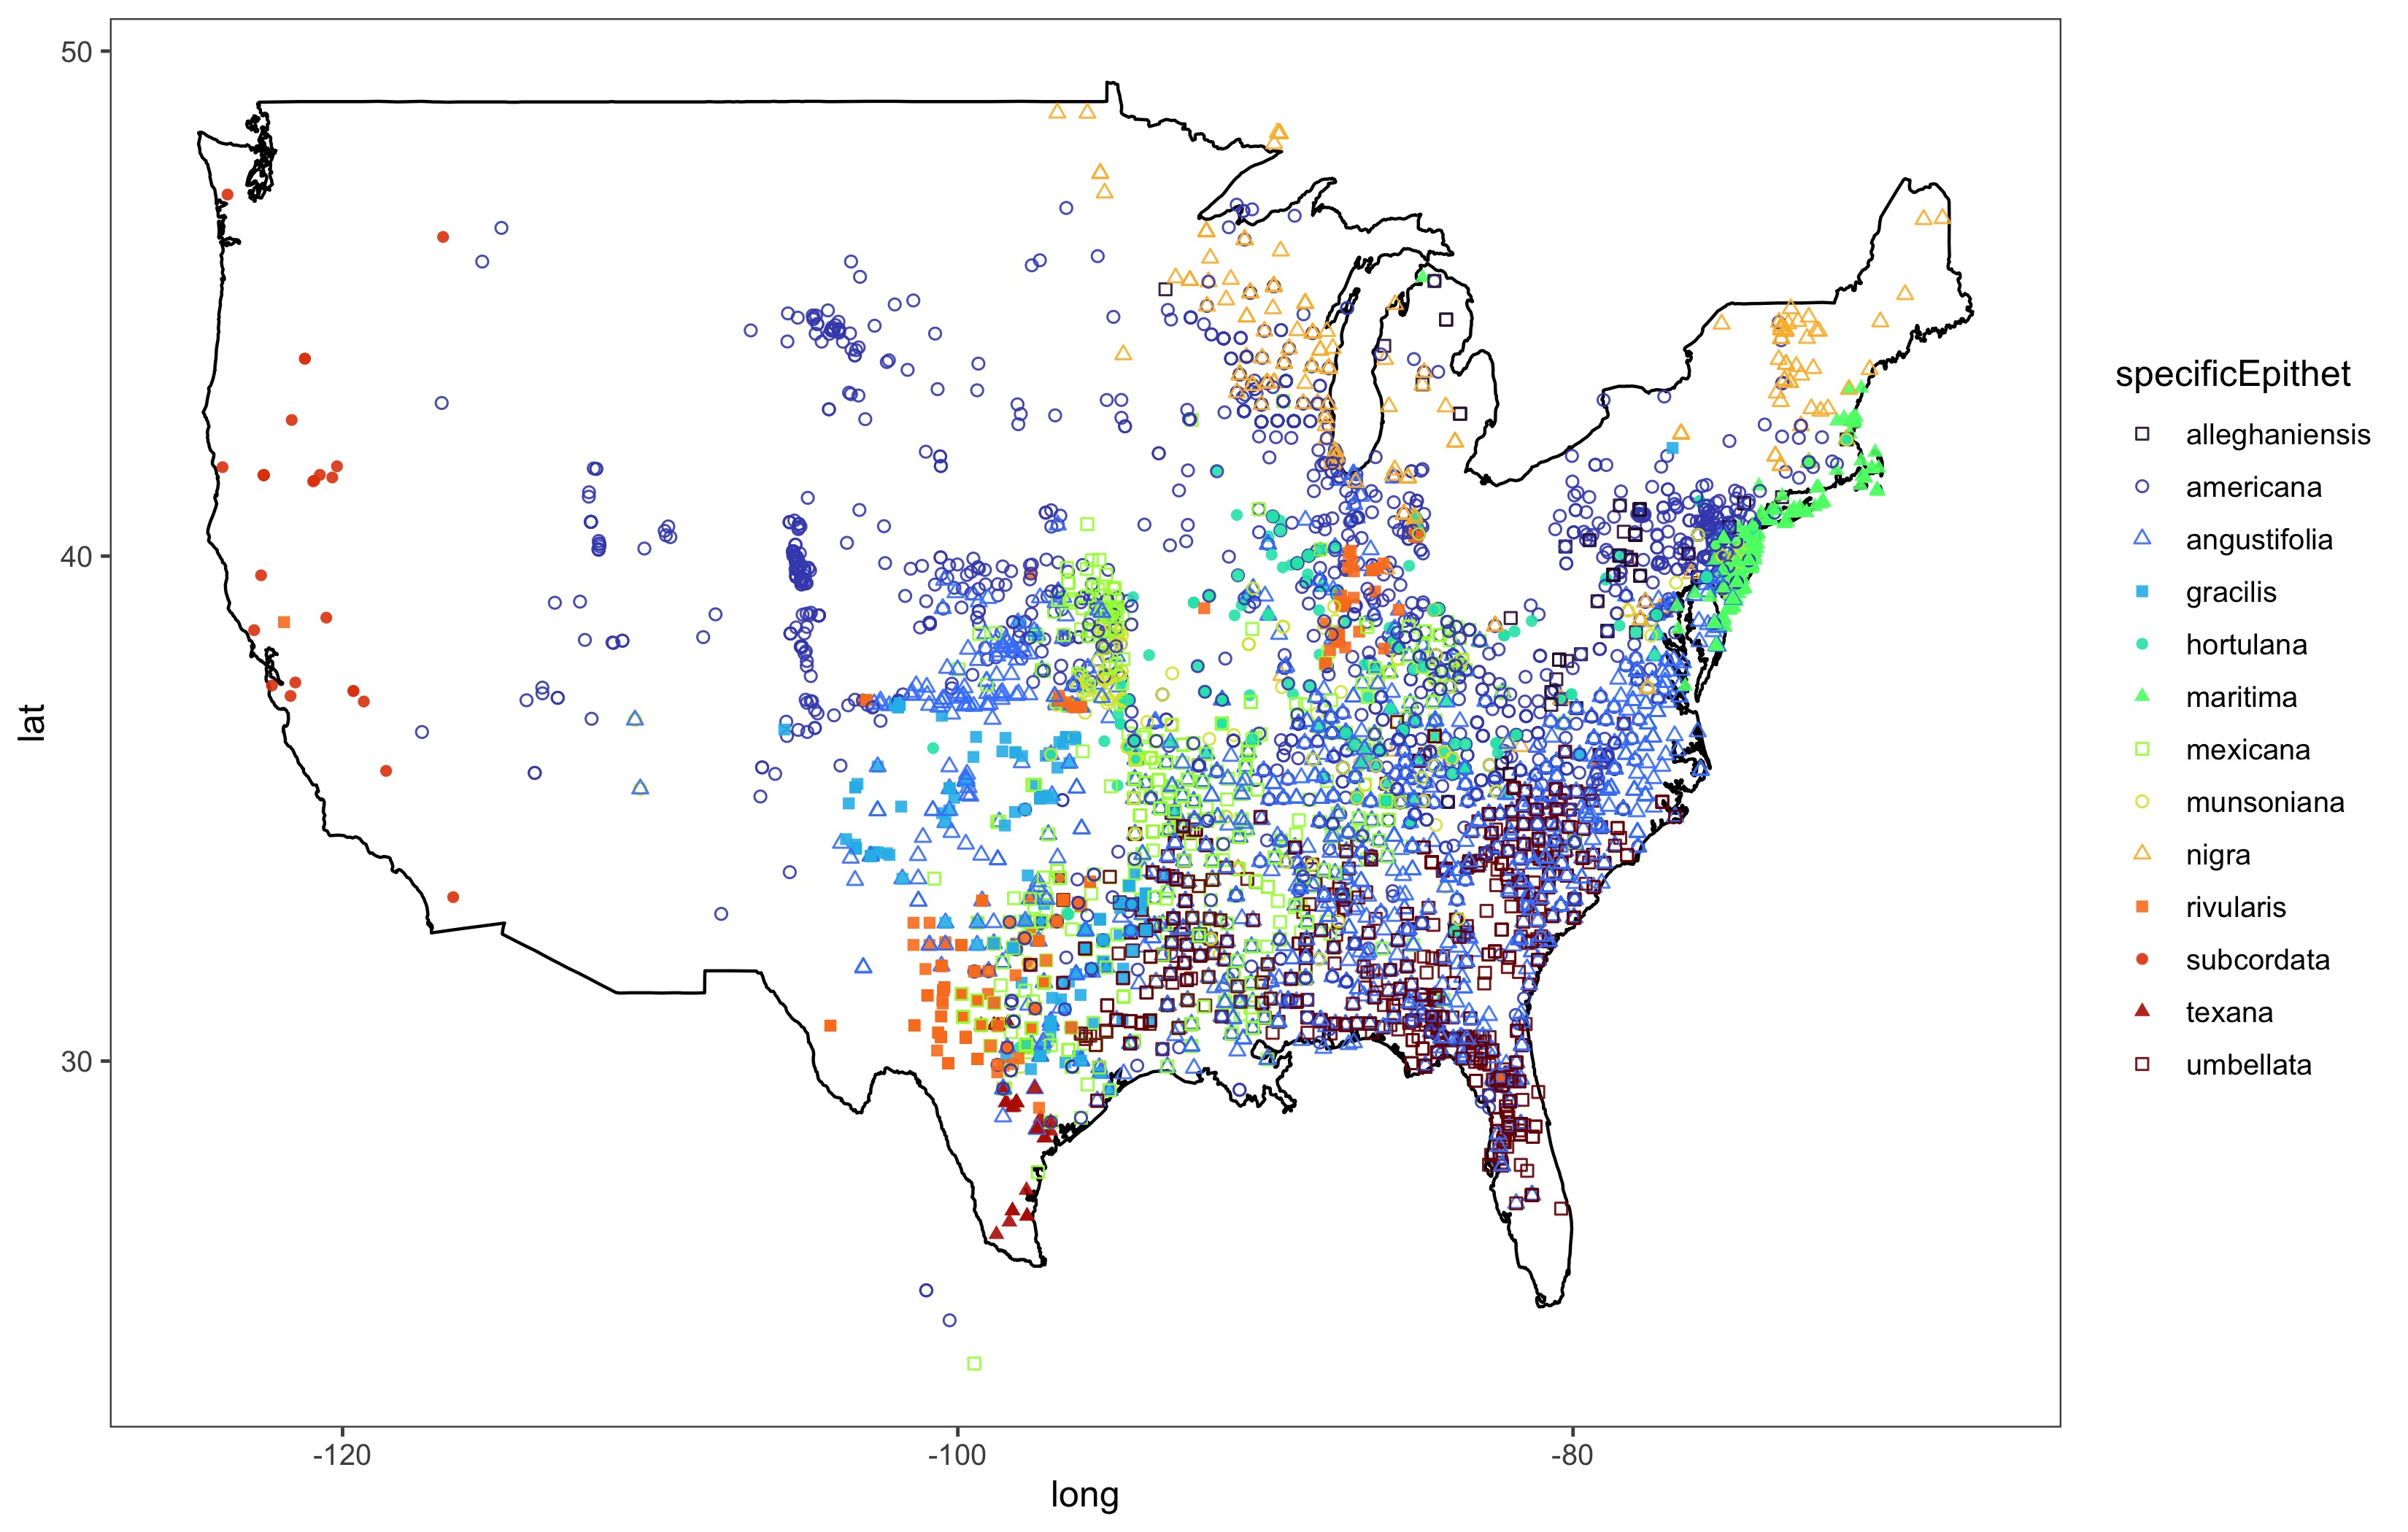
\includegraphics[width=\textwidth]{..//..//Plots/map.jpeg}
    \caption{Map to show where data come from and to point out the two never hysteranthy species are highly endemic}
    \label{fig:mappy}
\end{figure}

\begin{figure}[h!]
    \centering
 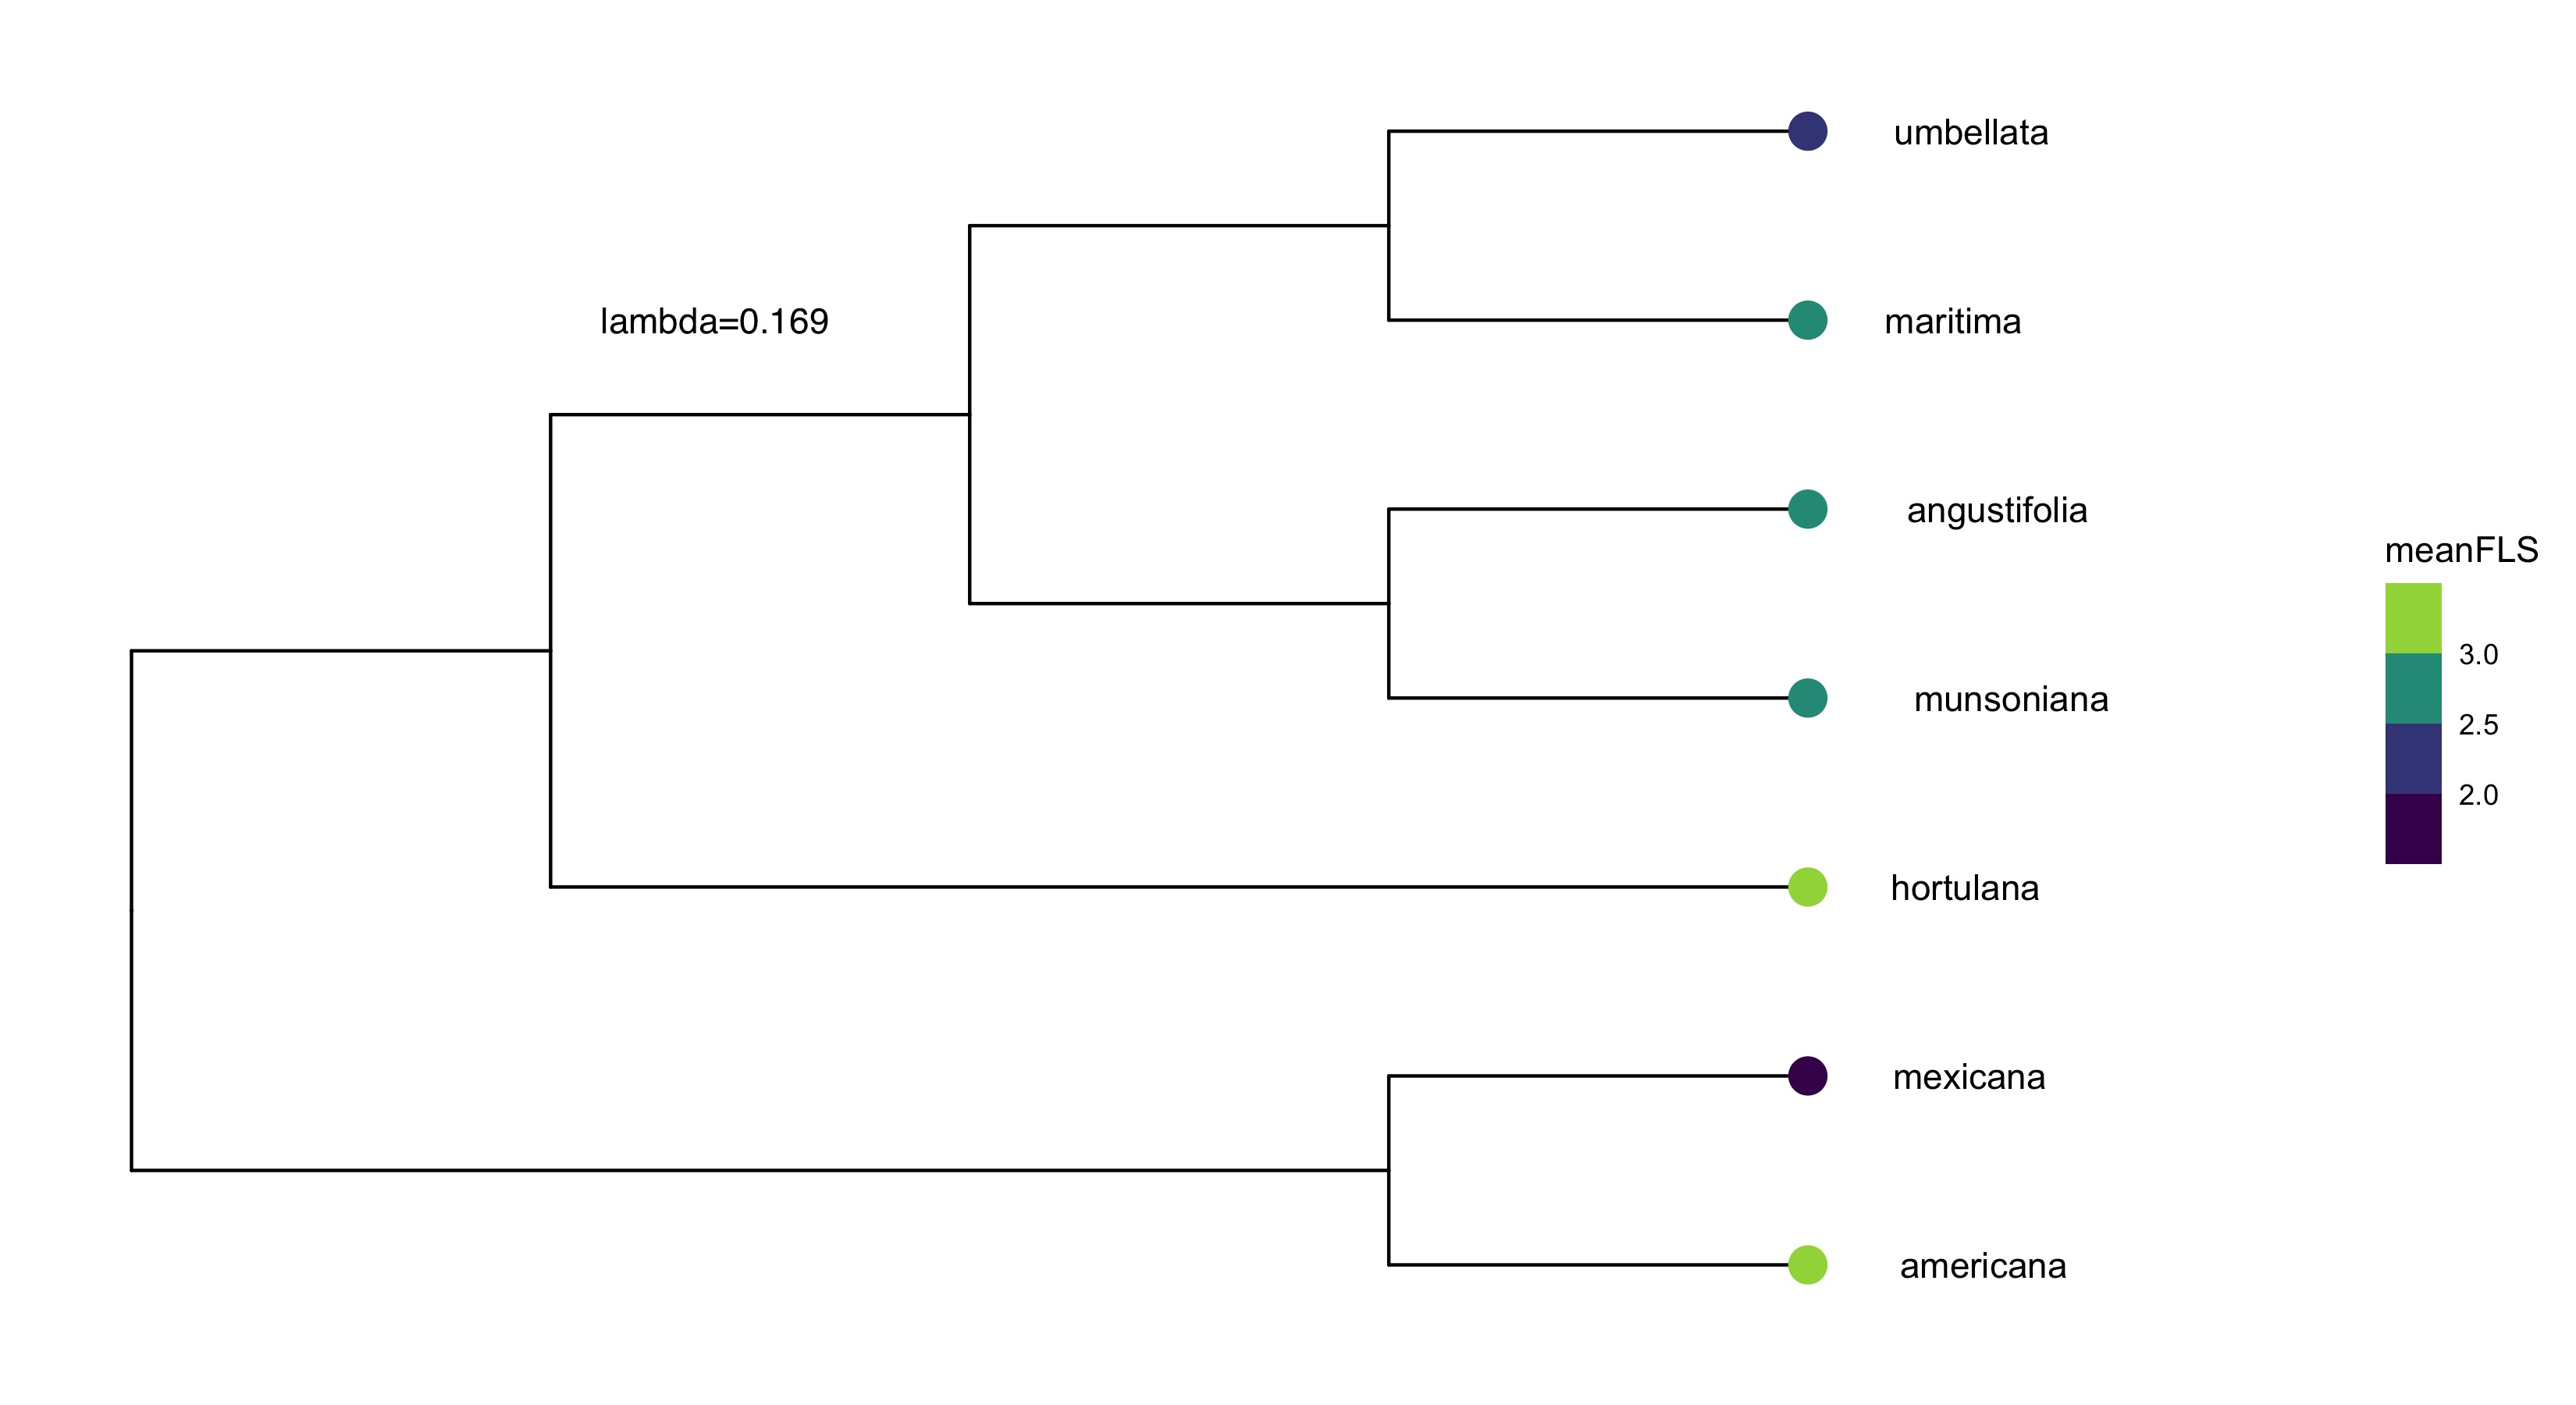
\includegraphics[width=\textwidth]{..//..//Plots/phylosig1.jpeg}
    \caption{place holder for the phylgenies: Ideally will have all N.A. Prunus \texit{and} Prunocerasus }
    \label{fig:phylo}
\end{figure}

\begin{figure}[h!]
    \centering
 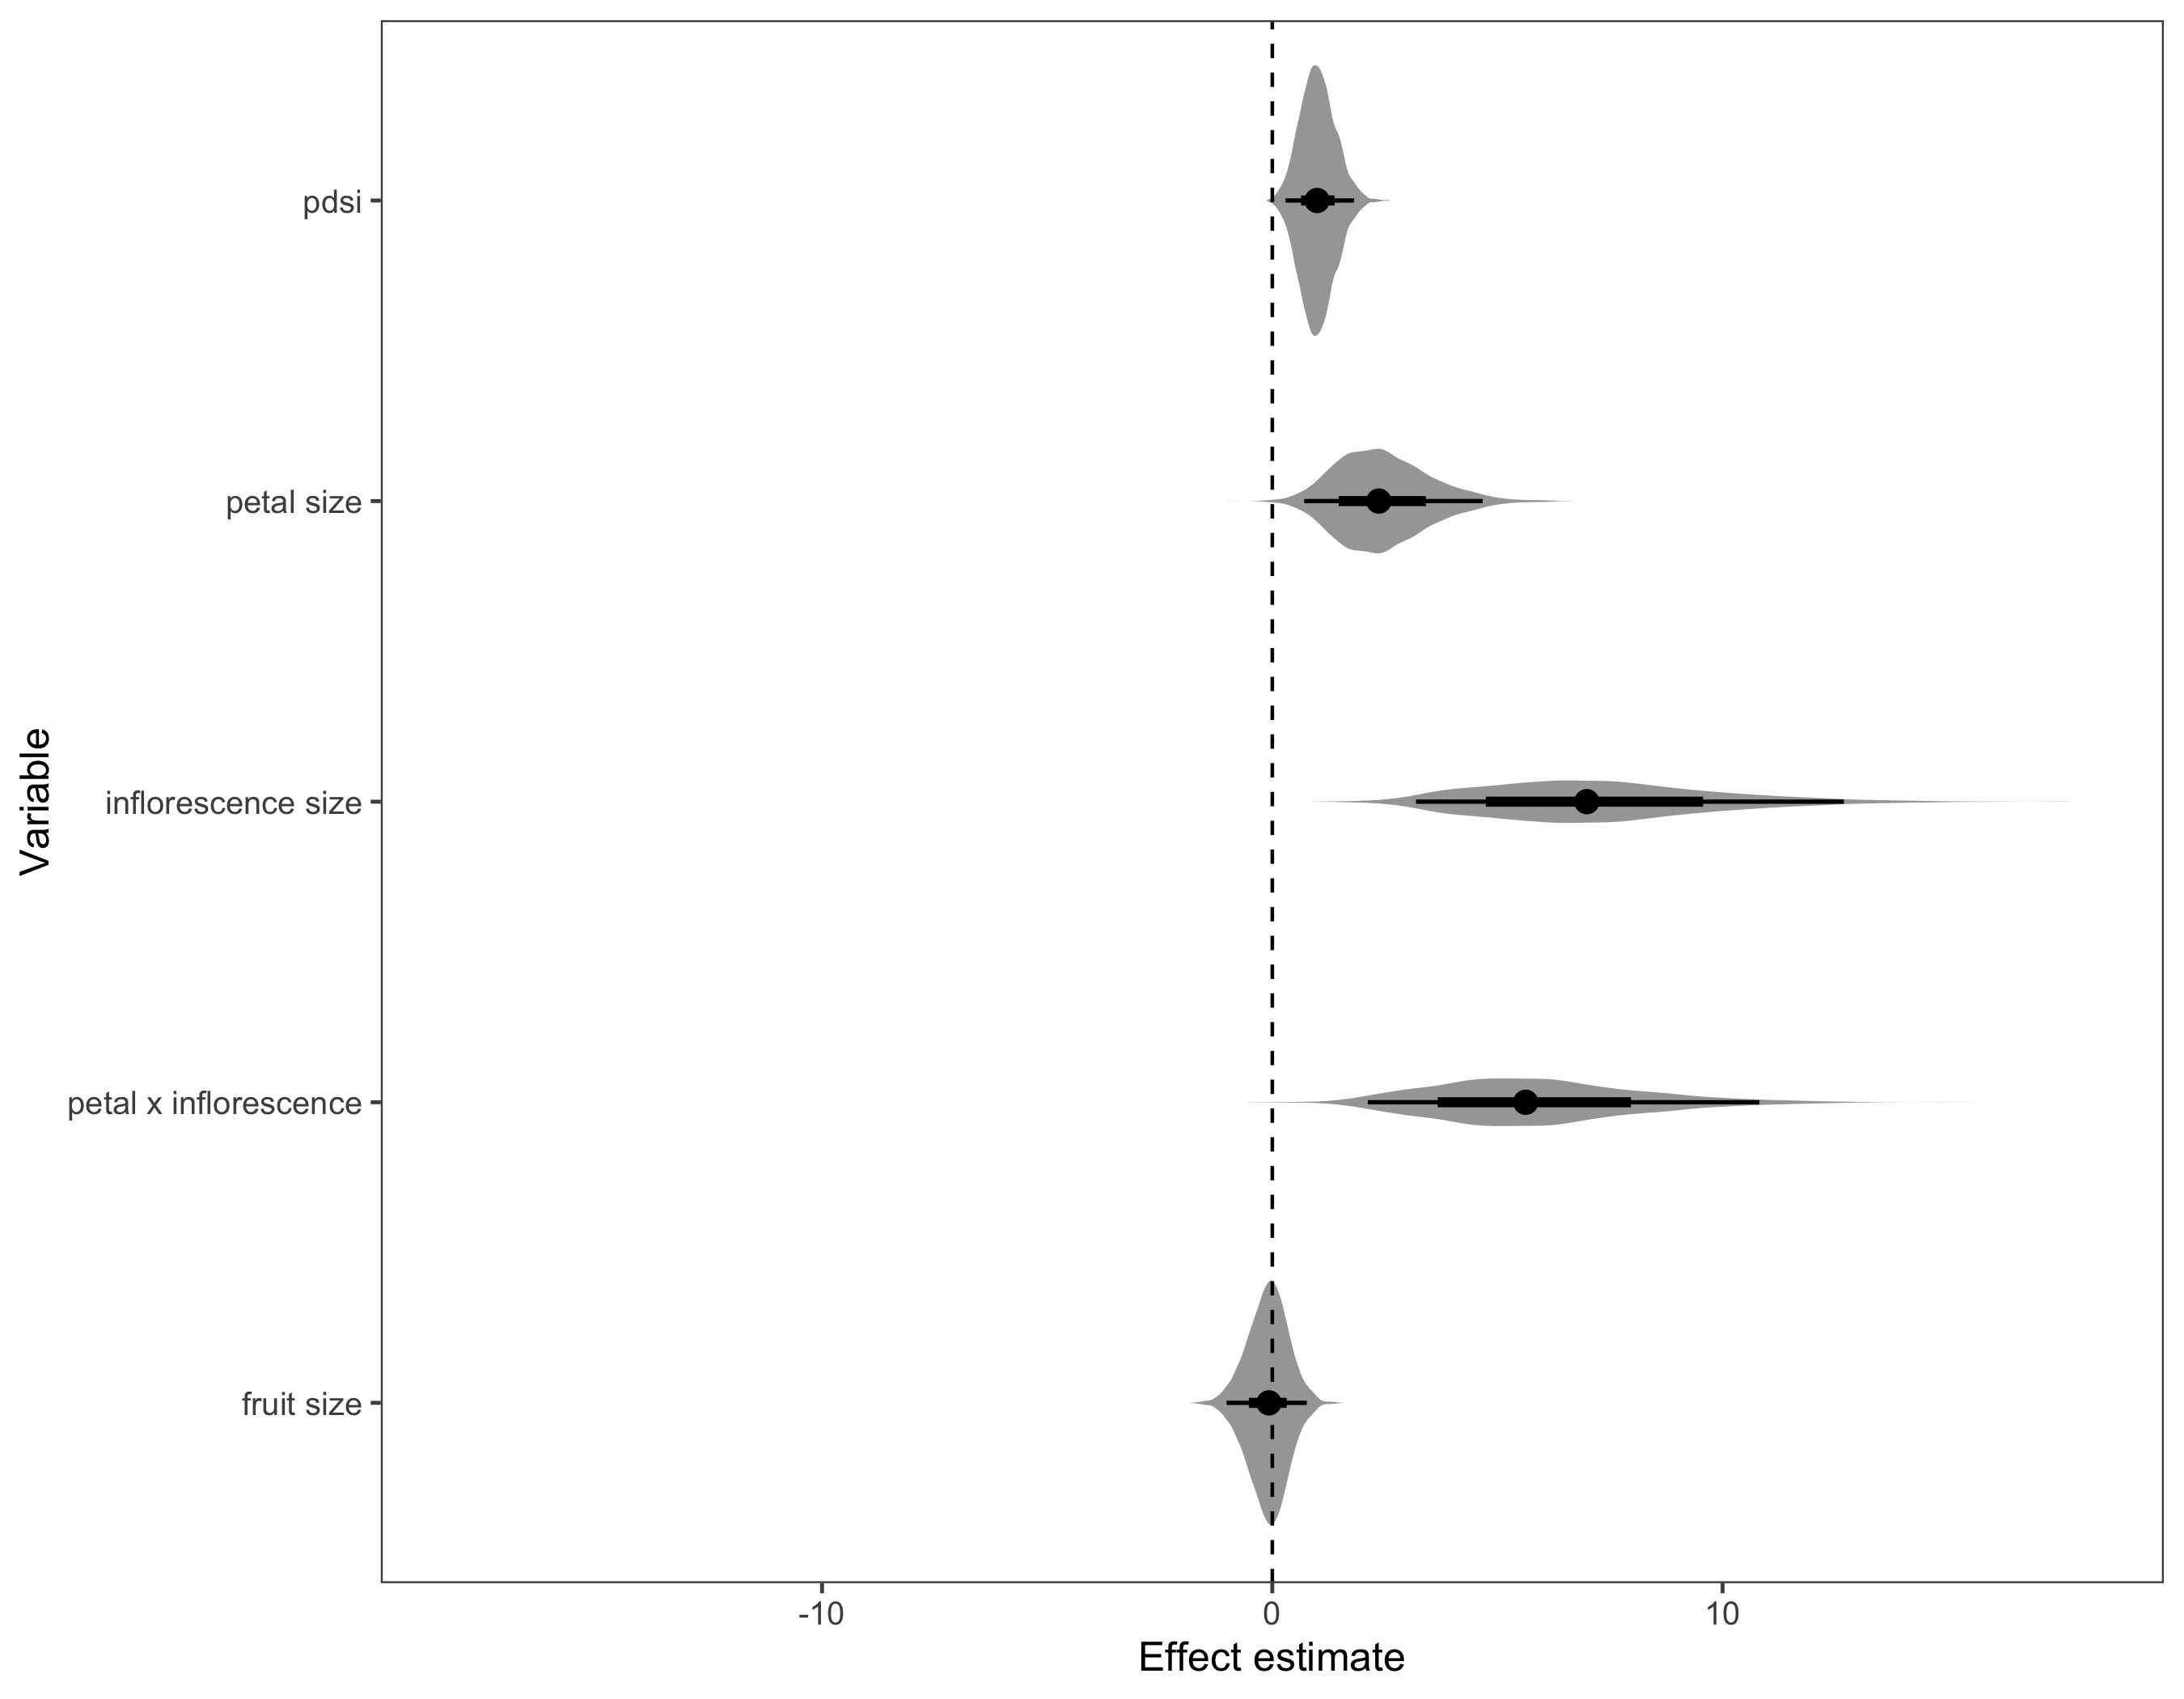
\includegraphics[width=\textwidth]{..//..//Plots/fullprunus_mus.jpeg}
    \caption{From the full genus analysis: Positive is less hysteranthus so aridity increases ihysteranthy, flower size decreases (ie smaller flowers- more hysteranthous) and no relationship with fruit size }
    \label{fig:cherries}
\end{figure}


\begin{figure}[h!]
    \centering
 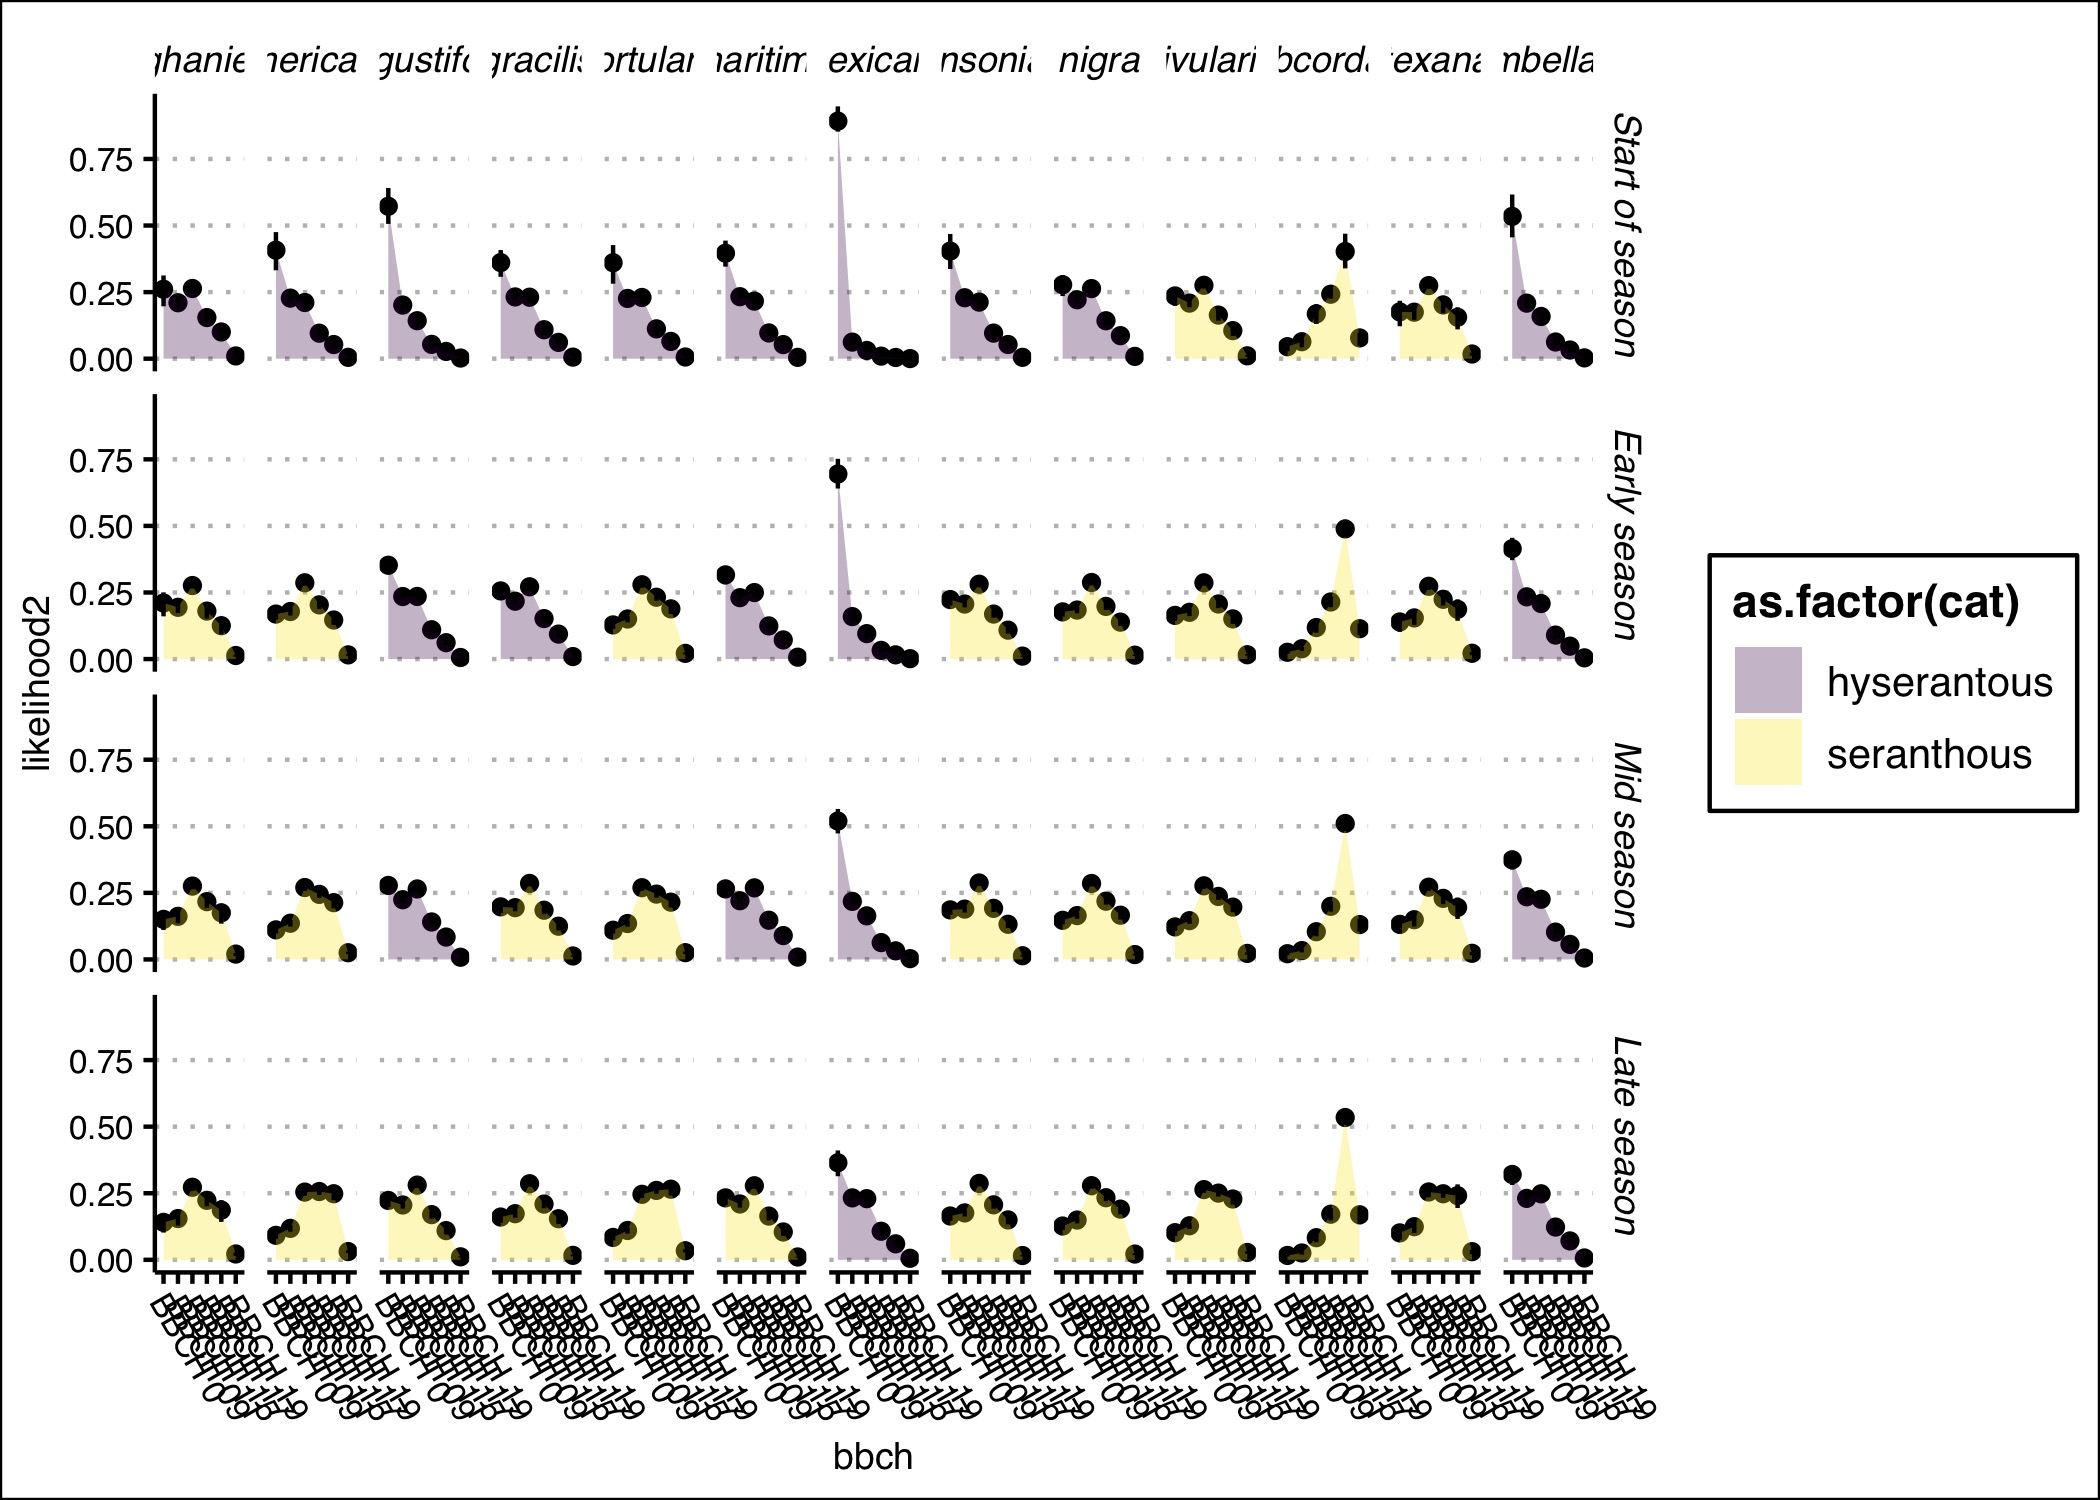
\includegraphics[width=\textwidth]{..//..//Plots/ord_quants.jpeg}
    \caption{ Likelihood of hysteranthy throughout the flowering season for each species in prunocerasus}
    \label{fig:plums}
\end{figure}

\begin{figure}[h!]
    \centering
 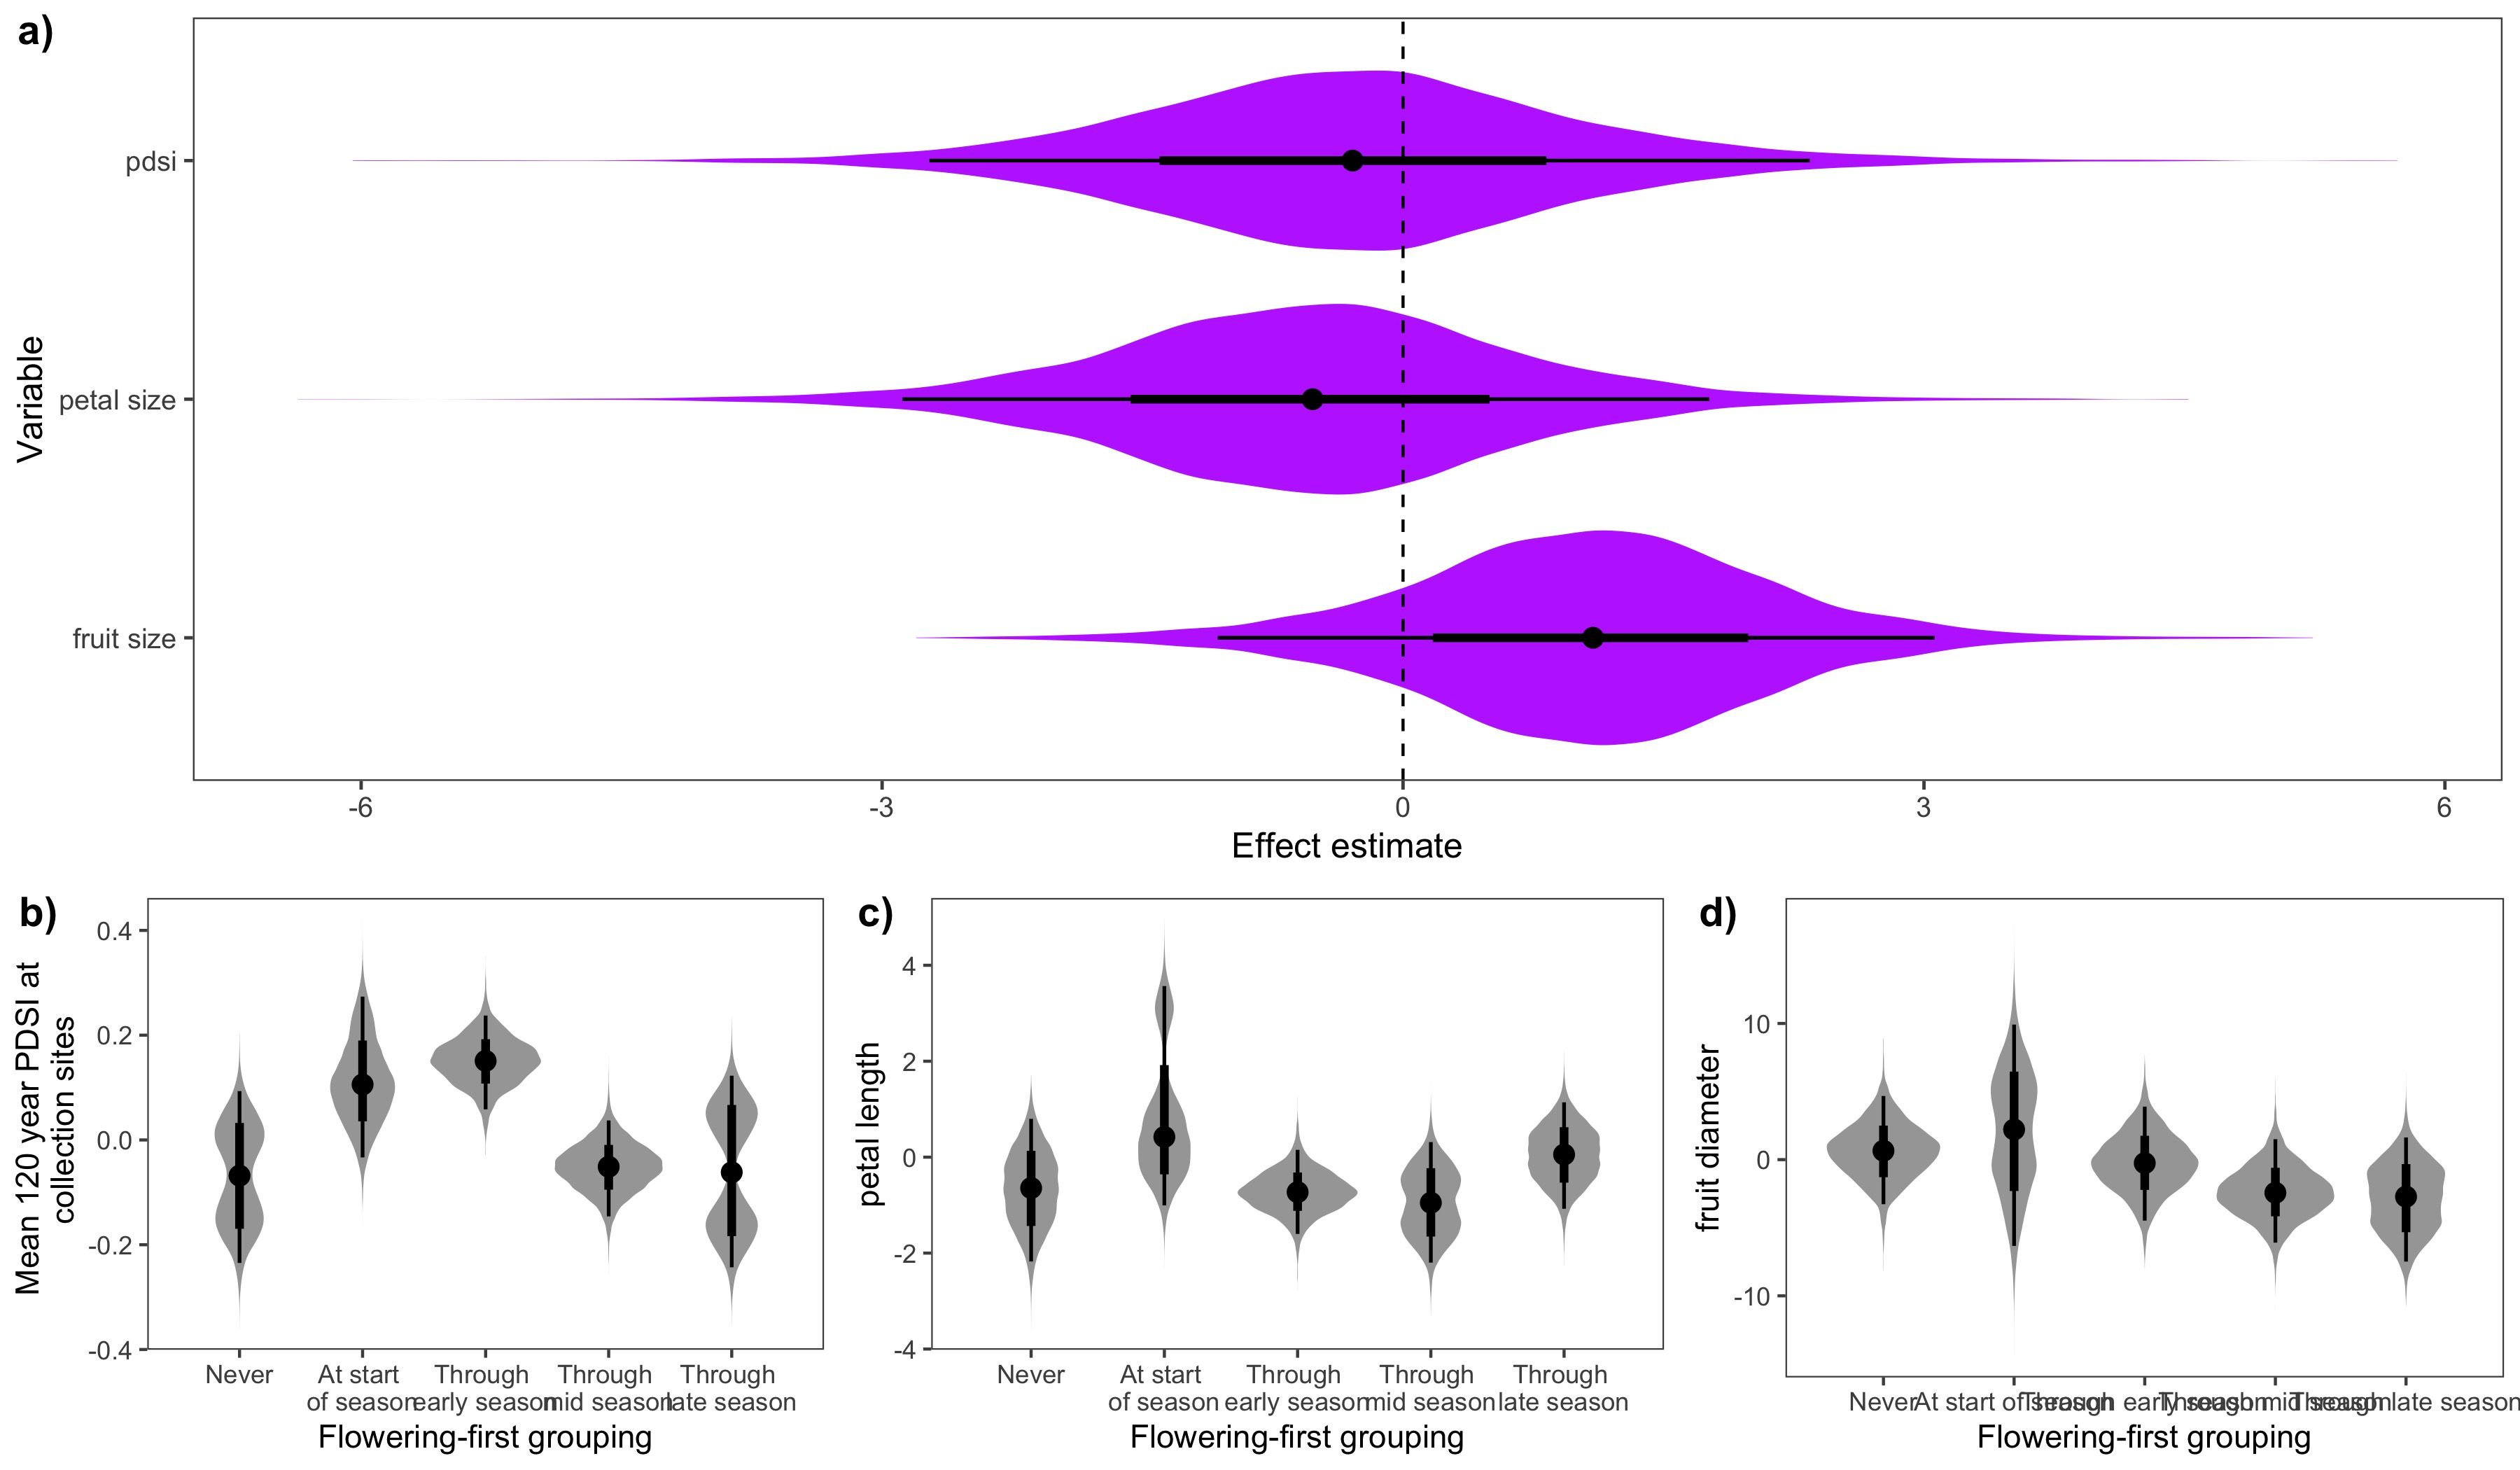
\includegraphics[width=\textwidth]{..//..//Plots/cerasus_mus.jpeg}
    \caption{Effect estimates. Why are they so different in prunucerasus? 1. measurement error model increases uncertainty. 2. outlyers have stronger influence. 3. Maybe too closely related (all flower to somedegree while leave are developing) }
    \label{fig:prunes}
\end{figure}


\begin{figure}[h!]
    \centering
 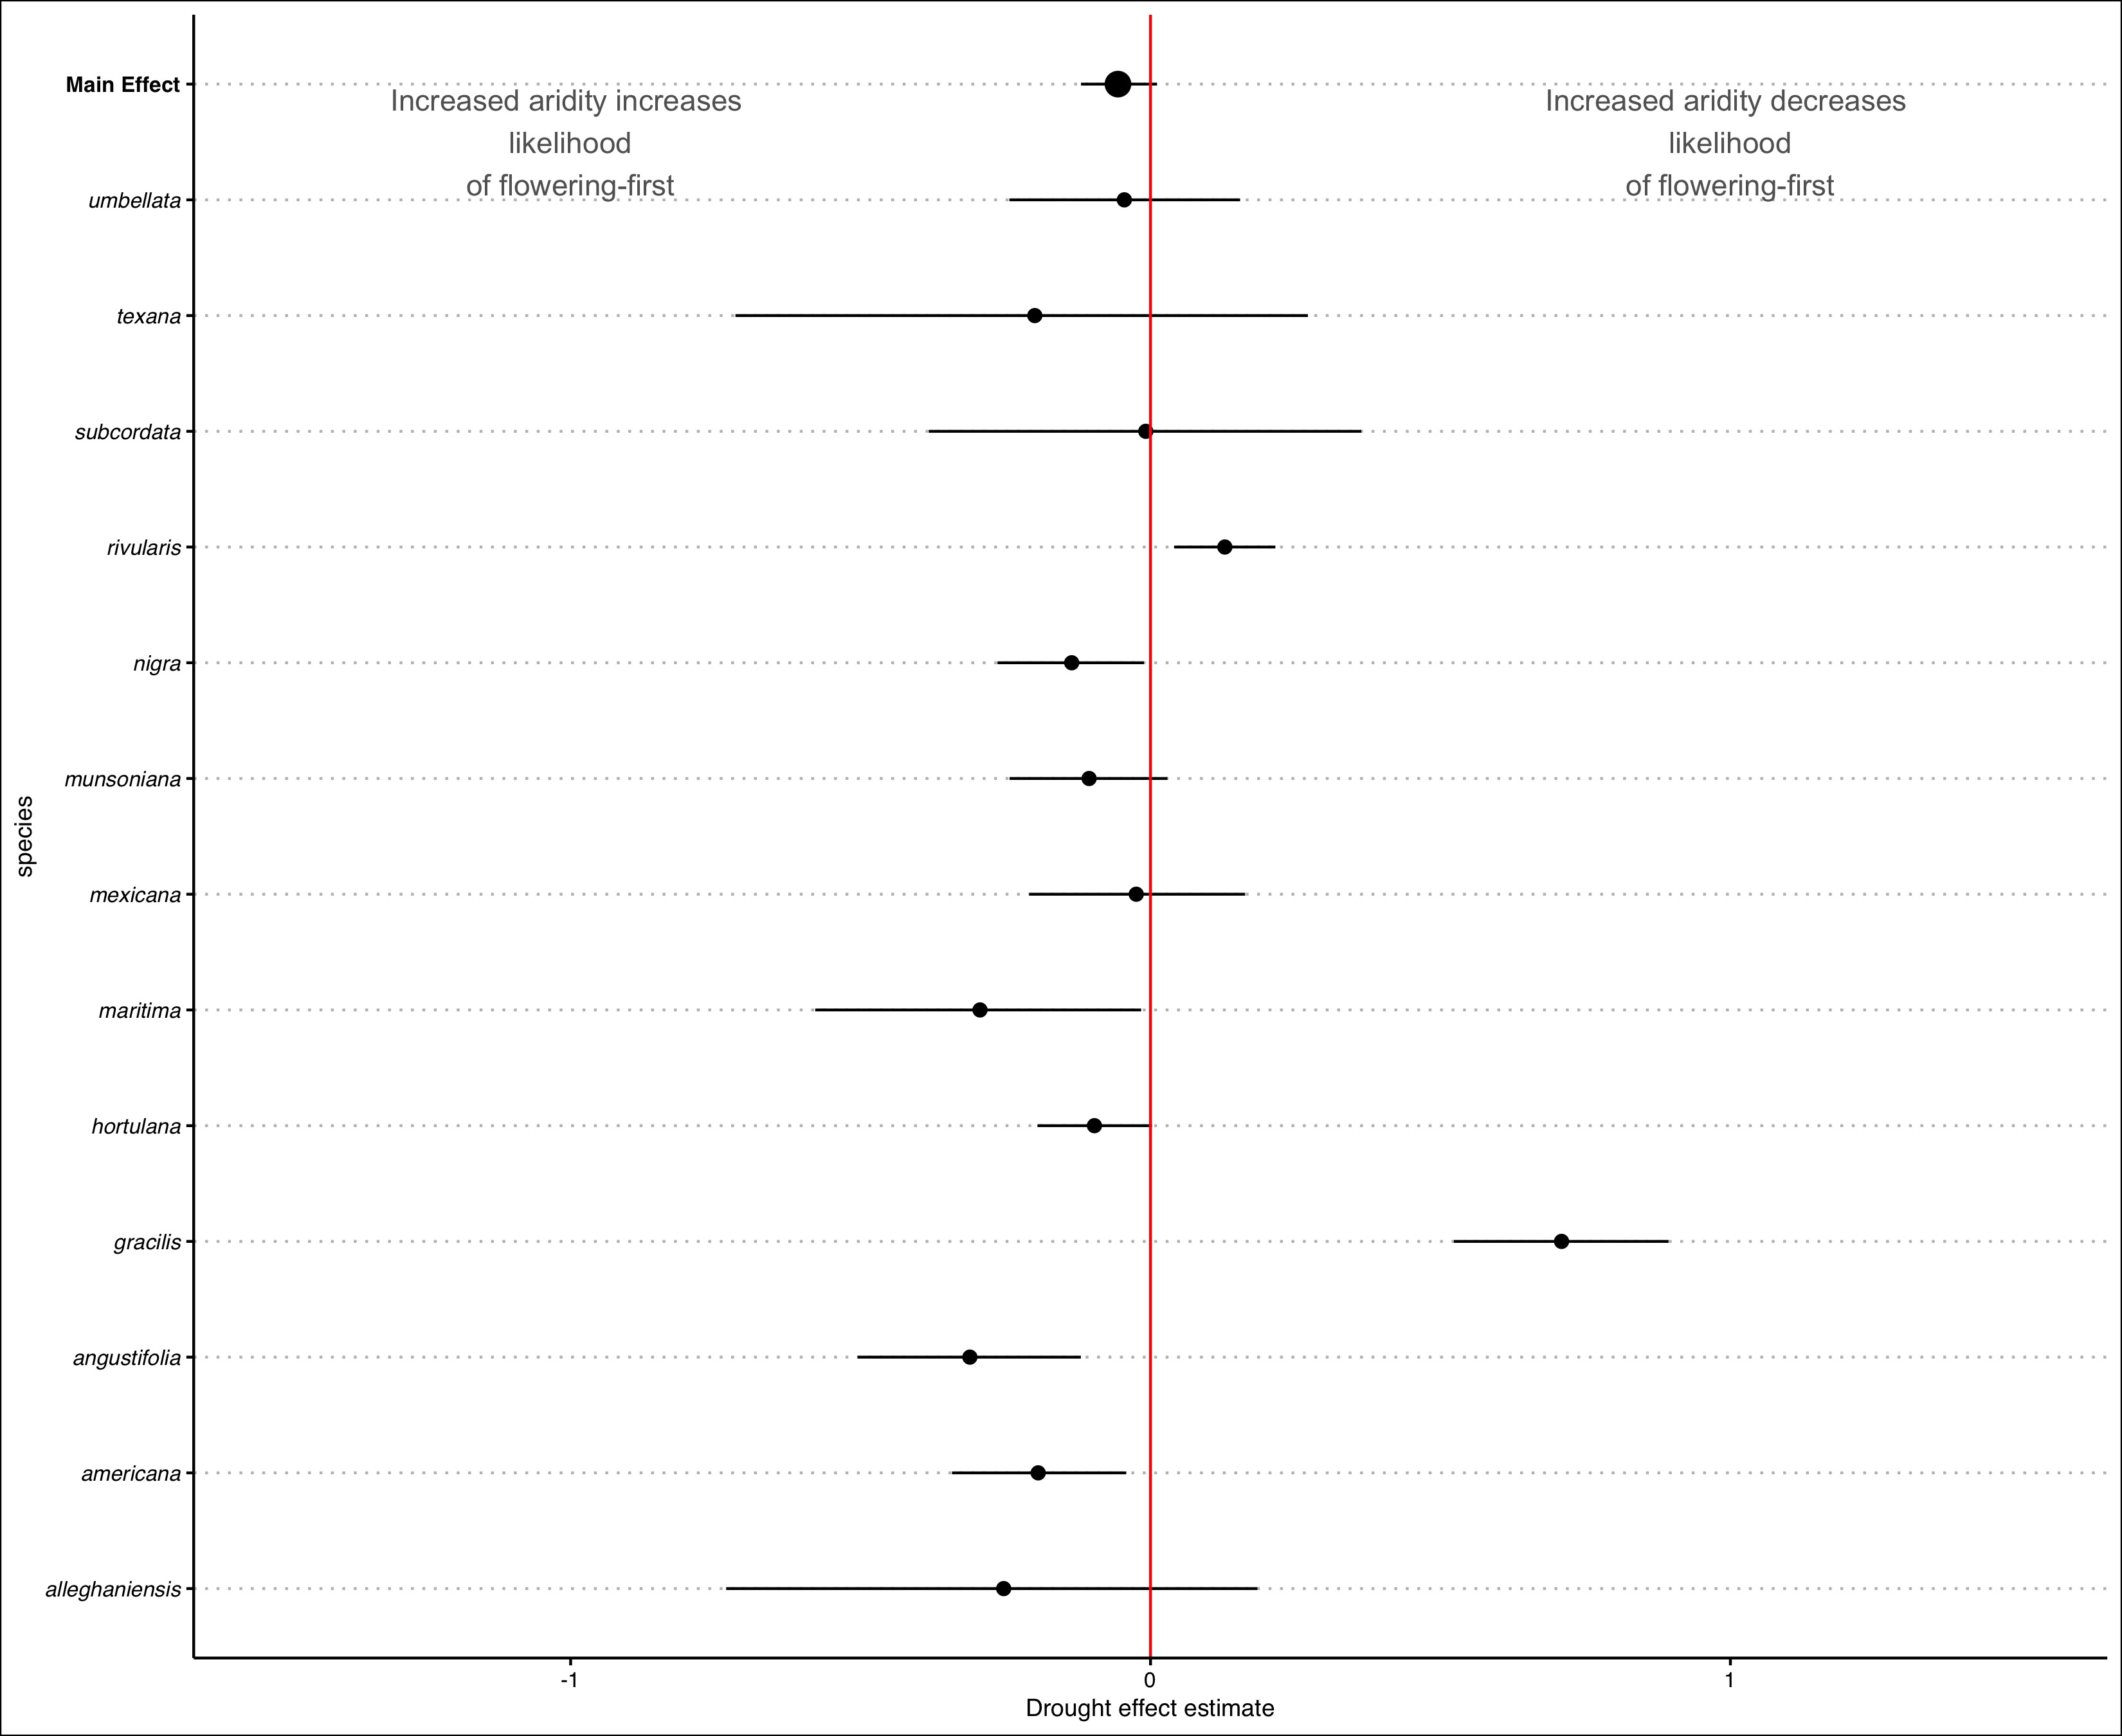
\includegraphics[width=\textwidth]{..//..//Plots/droughtstuff.jpg}
    \caption{Hysteranthy more likely in drought years.}
    \label{fig:plastic}
\end{figure}

\end{document}
